\section{Grundlagen}
\label{sec:basics}

In dieser Sektion werden die Technologien, welche die Grundlage für das Monitoring Tool darstellen, kurz erläutert. Für jede dieser Technologien wird die Motivation und die grundsätzliche Funktionalität erklärt.

\subsection{Power-over-Ethernet (PoE)}
\label{sec:poe}
Mit Power-over-Ethernet (PoE) ist es möglich, dass man Geräte über die oft schon vorhandenen Netzwerkkabel mit Strom versorgen kann. Die Idee dahinter, warum man sich überhaupt darüber Gedanken gemacht hat, war dass es eine Menge Geräte gibt die eigentlich eine geringe Stromversorgung brauchen, diesen Strom jedoch durch einen Anschluss an der Stromversorgung des Gebäudes tilgen. Was bedeutet: Überall wo man einfache Netzwerkgeräte braucht (Print-Server, Voice-over-IP Geräte, etc.) braucht man immer sowohl Netzwerk- als auch Stromkabel.

Mittels PoE können die zusätzlichen Stromkabel eingespart werden, sofern das Gerät eine Ladung über das Netzwerk-Interface erlaubt. Dies eignet sich sehr gut für einige eher einfache Geräte wie Webcams, Handhelds, etc.

Für PoE wurden bisher zwei IEEE Standards verabschiedet. Tabelle \ref{tab:compareIeee} zeigt einen kurzen Vergleich zwischen den beiden Standards.

\begin{table}[h]
 \centering
 \begin{tabular}{|c|c|c|c|}
   \hline
   \textbf{IEEE Nummer} & \textbf{Bezeichnung} & \textbf{Leistung / Port} & \textbf{nutzbare Leistung} \\
   \hline
   IEEE 802.3af & PoE & 15,4 Watt & ca. 12,9 Watt \\
   \hline
   IEEE 802.3at & PoE+ & 60 Watt & ca. 51 Watt \\
   \hline
 \end{tabular}
 \caption{Vergleich IEEE Standards \cite{poe2}}
 \label{tab:compareIeee}
\end{table}

Die nutzbare Leistung unterscheidet sich deshalb von der Leistung / Port, weil hier auch der Verlust der bei den RJ-45 Steckern passiert und auch den Verlust über eine Strecke von 100 Metern eingerechnet wurde.

\subsubsection{IEEE 802.3af}
Dieser Standard funktioniert nur mit 10Base-T und 100Base-TX Verbindungen. Die Idee hinter diesem Standard ist, dass man die freien Aderpaare (bei diesen beiden Verbindungen werden nur 2 der 4 Paare verwendet) für die Stromübertragung verwendet. Dieses Verfahren wird \emph{Spare-Pairs-Verfahren} genannt. Abbildung \ref{fig:spare-pairs} zeigt den Aufbau dieses Verfahrens.

\begin{figure}[h]
    \centering
    \leavevmode
    \includegraphics[width=1.0\linewidth]{figures/spare-pairs-verfahren-marked}
    \caption{Spare-Pairs-Verfahren\cite{poe1}}
    \label{fig:spare-pairs}
\end{figure}

Es gibt diesen Standard in verschiedenen Klassen. Die Default Klasse entspricht den oben beschriebenen Spezifikationen. Die anderen Klassen können teilweise auch mehr Leistung bereit stellen (bis zu ca. 21 Watt). Es gibt auch Switches, welche ca. 30 Watt pro Port bereit stellen, diese verhalten sich jedoch nicht dem Standard entsprechend.

\subsubsection{IEEE 802.3at}
Dieser Standard ist auch bei 1000Base-T Verbindungen anwendbar. Hier wird der Strom nicht in den unbenutzten Aderpaaren übertragen (die gibt es hier ja nicht), sondern der Strom wird mit den zu übertragenden Daten überlagert und somit übertragen. Dieses Verfahren wird \emph{Phantom-Speisung} genannt. Abbildung \ref{fig:phantom-speisung} zeigt den Aufbau dieses Verfahrens.

\begin{figure}[h]
    \centering
    \leavevmode
    \includegraphics[width=1.0\linewidth]{figures/phantom-speisung-marked}
    \caption{Phantom-Speisung \cite{poe1}}
    \label{fig:phantom-speisung}
\end{figure}

Dieser Standard bietet höhere nutzbare Leistung, braucht aber auch bessere Kabel um richtig zu funktionieren.

\subsubsection{Energieversorgung}

Für die Versorgung der Kabel mit Strom, um sie beim Empfänger benutzen zu können, gibt es zwei Möglichkeiten\cite{poe2}:
\begin{description}
 \item[Endspan -] Es gibt direkt einen Switch welcher die Ports mit Energie versorgt.
 \item[Midspan -]Man baut auf halber Strecke (deshalb Midspan) ein zusätzliches Gerät in das Netzwerk ein, welches die Leitung mit Energie versorgt. Dies ist notwendig, solange man PoE in einen Bereich einsetzen will, in dem es noch keine PoE-fähigen Switche gibt. Das zusätzlich installierte Gerät wird auch Injector genannt.
\end{description}

Wichtiger Punkt hier ist noch, dass ein PoE Switch keine Geräte beschädigen darf, die angeschlossen sind, jedoch kein PoE unterstützen. Hierfür ist es notwendig, dass der PoE Switch erkennen kann ob ein angeschlossenes Gerät mittels PoE mit Energie versorgt werden soll oder nicht. Um dies zu gewährleisten, wurde in den IEEE Standards eine Stufe in der Kommunikationsaufbauphase hinzugefügt.

Hier wird mit kleiner Stromstärke geprüft ob der Empfänger einen gewissen Stromwiderstand hat (die Bereiche sind genau definiert). Falls ja, wird geprüft welcher PoE Standard verwendet werden soll. Danach beginnt die Speisung mit Strom und die Datenverbindung wird aufgebaut.

\subsection{SNMP}
\label{sec:SNMP}
Simple Network Management Protocol (SNMP) ist ein in RFC 1157 definiertes Protokoll zur Überwachung und zum Management von Netzwerkkomponenten.\cite{rfc1157} In RFC 3410 werden Erweiterungen definiert, die als SNMPv3 aktueller De-facto-Standard sind.\cite{rfc3410}

Das Protokoll zielte darauf ab, eine schnell zu implementierende und einfache Lösung für das Management von Netzwerkkomponenten zu erhalten. Bei der Definition von SNMP wurden daher Abstriche beispielsweise hinsichtlich der Sicherheit in Kauf genommen. In SNMPv3 wurden diesbezüglich einige Verbesserungen vorgenommen.

Bei SNMP wird zwischen zwei Entitäten unterschieden, Manager und Agents. Manager, oft auch als Network Management Stations (NMS) bezeichnet, sind für das Abrufen und Empfangen von Informationen über SNMP verantwortlich.\cite{essential-SNMP} Agents sind Software-Artefakte, die auf den Netzwerkkomponenten ausgeführt werden. Ihre Aufgabe ist es, Managern Daten zur Verfügung zu stellen oder diese an die Manager zu senden. Abfragen des Managers an den Agent werden als Query bezeichnet. Unter Trap versteht man eine asynchrone Übermittlung des Agenten an den Manager, nachdem der Agent den Eintritt eines vordefinierten Ereignisses festgestellt hat. Bild \ref*{fig:snmp-schema} stellt die Beziehung der beiden Enitäten zu einander schematisch dar.

\begin{figure}[tbph]
\centering
\includegraphics[width=0.7\linewidth]{./figures/snmp-schema}
\caption{Schema der Manager/Agent-Beziehung, aus \cite{essential-SNMP}}
\label{fig:snmp-schema}
\end{figure}

Die vom Agent verfügbar gemachten Daten sind in als Baum aufgebauten Datenbanken, den sogenannten Management Information Base(s) (MIB), definiert. Ein Agent kann dabei mehrere MIBs implementieren.\cite{essential-SNMP} Die Informationen stehen dabei in den Blättern des Baums zur Verfügung. Die Knoten dienen zur Organisation des Baums. Der Zugriff auf ein Blatt erfolgt anhand von eindeutigen Object Identifiern (OID), die einen Pfad im Baum zum gewünschten Blatt darstellen. Abbildung \ref{fig:snmptree} zeigt beispielhaft, wie ein solcher Baum aussehen könnte. In diesem Baum gibt es insgesamt sechs Blätter, es kann somit auf sechs Daten zugegriffen werden. Die OID 1.3.17.18 verweist hierbei auf das mittlere Blatt des rechten Astes. Neben den OIDs werden in MIBs weitere Informationen wie zum Beispiel ein sprechender Name und ein Datentyp für das jeweilig beschriebene Objekt festgelegt.

\begin{figure}[H]
  \begin{center}
    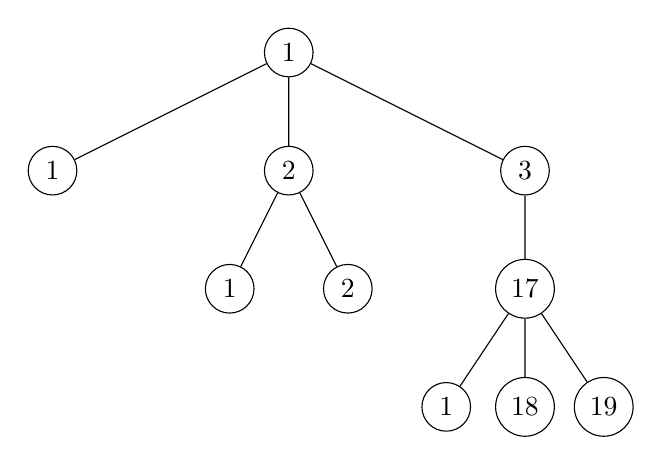
\begin{tikzpicture}[level/.style={sibling distance=30mm/#1}]
      \node [circle,draw] {$1$}
        child {node [circle,draw] {$1$}}
        child {node [circle,draw] {$2$}
          child {node [circle,draw] {$1$}}
          child {node [circle,draw] {$2$}}
        }
        child {node [circle,draw] {$3$}
          child {node [circle,draw] {$17$}
            child {node [circle,draw] {$1$}}
            child {node [circle,draw] {$18$}}
            child {node [circle,draw] {$19$}}
         }
       };
    \end{tikzpicture}
    \caption{Beispiel eines MIB Baumes}
    \label{fig:snmptree}
  \end{center}
\end{figure}

Die Kommunikation zwischen Manager und Agent erfolgt über Protocol Data Units (PDUs), die das Nachrichtenformat der Kommunikation festlegen.\cite{essential-SNMP} Die wichtigsten fünf PDUs sind die folgenden:

\begin{description}
  \item[GET REQUEST:] Anfrage des Managers an den Agent. Der Agent beantwortet die Anfrage mit einem \textbf{GET RESPONSE}.
  \item[GET RESPONSE:] Antwort eines Agents auf eine Anfrage.
  \item[SET REQUEST:] Manager fordert einen Agent zur Änderung eines Wertes auf. Als Antwort erhält der Manager ein \textbf{GET RESPONSE} vom Agent. Im Fehlerfall wird dem Manager darin ein Fehlercode übermittelt.
  \item[GET\_NEXT REQUEST:] Manager forder jenen Wert im Baum an, der als nächstes aufgelistet ist. Dabei wird eine Tiefensuche angewendet. Der Agent beantwortet die Anfrage mit einem \textbf{GET RESPONSE}. Hierbei ist jedoch zu beachten, dass dieser Wert nicht zwingend der tatsächlich gewünschte Wert ist. Existiert das gewünschte Blatt nicht, liefert die Anfrage trotzdem das Datum des nächsten Knotens.
  \item[TRAP:] Im Eintrittsfall eines vordefinierten Ereignisses sendet der Agent an einen zuvor konfigurierten Manager eine Nachricht. Der Agent erhält hierbei keinerlei Bestätigung über den Empfang der Trap.
\end{description}

